% Basic document setup
% 7"×10" format with appropriate margins
\usepackage[paperwidth=7in, paperheight=10in, margin=0.75in, inner=0.875in, outer=0.625in]{geometry}
\usepackage[latin]{babel}
\usepackage{graphicx}
\usepackage{booktabs}
\usepackage{epstopdf}
\usepackage{float}
\usepackage{tikz}
\usepackage{pgfplots}
\usepackage{pgffor}
\usepackage{enumitem}
\usepackage{tabularx}
\usepackage{graphicx}
\usepackage{changepage}
\usepackage{verbatim}
\usepackage{comment}
\usepackage{setspace}
\usepackage{ragged2e}
\usepackage{array}
\usepackage{pgffor} % Required for \foreach
\usepackage{ifoddpage}
\usepackage{catchfile} 
\usepackage{xstring}
\usepackage[most]{tcolorbox}  % Ensure this is included in your preamble
\usepackage{array}
\usepackage{colortbl}
\usepackage{caption}
\usepackage{varwidth}
\usepackage{pagecolor}
\usepackage{lipsum} % optional for filler text
\usepackage{eso-pic} % For background picture in sidenotes



\pgfplotsset{compat=1.18}

% Typography and text formatting
\usepackage[protrusion=true,expansion=true]{microtype}
\usepackage{CJK}
\newcommand{\katakana}[1]{\begin{CJK}{UTF8}{min}#1\end{CJK}}
\usepackage{shadowtext}
\usepackage{bbding}
\usepackage{textcomp}
\usepackage{hyperref}
\usepackage{parskip}
\usepackage{multicol}
\usepackage{needspace}
\usepackage{etoolbox}
\usepackage{pifont}  % for nice symbols like the filled circle

% Math packages
\usepackage{amsmath, amssymb, physics}
\usepackage{unicode-math}

% Multilingual support
\usepackage{polyglossia}
\usepackage{amsfonts}
\usepackage{lmodern} 
\setdefaultlanguage{english}
\setotherlanguage{greek}
\setotherlanguage{hebrew}
\setotherlanguage{sanskrit}

% Assign fonts to polyglossia languages
\newfontfamily\greekfont[Script=Greek]{Linux Libertine O}
\newfontfamily\hebrewfont[Script=Hebrew]{Arial Hebrew}
\newfontfamily\sanskritfont[Script=Devanagari]{Devanagari Sangam MN}

% Font configuration
\usepackage{fontspec}
\setmainfont{Libertinus Serif}                    % Main serif font
\newfontfamily\historyfont{Crimson Pro}           % Historical section font
          % Technical section font
\newfontfamily\commentaryfont{Crimson Pro}        % Commentary font


\newfontfamily\piefontfamily{Charis SIL}
\newfontfamily\ipafontfamily{Charis SIL}

% Create properly scoped commands that preserve current font size
\newcommand{\piefont}[1]{{\piefontfamily #1}}
\newcommand{\ipafont}[1]{{\ipafontfamily #1}}

\newfontfamily\summaryfont{Libertinus Serif Italic} % Summary font
\newfontfamily\technicalfont[ItalicFont={XITS Math}]{XITS Math}

% Color definitions
\usepackage{xcolor}
\definecolor{historycolor}{RGB}{70,30,0}         % Warm brown for historical sections
\definecolor{technicalcolor}{RGB}{0,20,60}       % Deep blue for technical sections
\definecolor{commentarycolor}{RGB}{0,0,0}        % Black for commentary
\definecolor{summarycolor}{RGB}{90,90,90}        % Gray for summaries
\definecolor{linkcolor}{RGB}{0,85,155}           % Link color for hyperlinks
\definecolor{SUMMARYCOLOR}{RGB}{90,90,90}        % Gray for summaries (uppercase)
\definecolor{lavender}{RGB}{230,230,250}
\definecolor{lightgray}{gray}{0.85}


% Section styling with titlesec
\usepackage{titlesec}
\usepackage{tocloft}  % For customizing TOC

\titleformat{\chapter}[hang]
    {\normalfont\huge\bfseries}{\thechapter}{1em}{} % Chapter title styling
\titlespacing*{\chapter}{0pt}{0pt}{10pt}            % Adjust spacing around chapters
\titleformat{\section}[hang]
    {\normalfont\Large\bfseries}{\thesection}{1em}{} % Section title styling
\titlespacing*{\section}{0pt}{10pt}{5pt}             % Adjust spacing around sections

% Frame and box packages
\usepackage[framemethod=TikZ,skipabove=6pt,skipbelow=6pt]{mdframed}
\usetikzlibrary{decorations.pathmorphing, decorations.shapes, decorations.footprints, shapes.geometric, positioning, patterns, fit,arrows.meta, decorations.pathmorphing, backgrounds, calc, decorations.fractals}
\mdfsetup{splitbottomskip=2pt, splittopskip=2pt}

\usetikzlibrary{lindenmayersystems}

% Spacing and layout settings
\setlength{\parindent}{0pt}      % No paragraph indentation
\setlength{\parskip}{0.5em}      % Paragraph spacing for better readability
\setlength{\columnsep}{15pt}     % Adjust column separation for multicol layout


% Force content to start on the next even-numbered page

\newcommand{\startchapter}{%
  \clearpage
  \checkoddpage
  \ifoddpage
    % already odd — do nothing
  \else
    \hbox{}
    \thispagestyle{empty}
    \clearpage
  \fi
}




% TOC customization for chapter summaries
\setlength{\cftbeforechapskip}{1.0em}  % Increase space between TOC entries
\setlength{\cftchapindent}{0em}        % Chapter indent in TOC
\renewcommand{\cftchapfont}{\bfseries} % Chapter font in TOC

% Header setup with fancyhdr - MUST be loaded after titlesec
\usepackage{fancyhdr}
\setlength{\headheight}{14pt}  % Slightly more than the required 13.59999pt

% Create chapter title extraction command to handle only the title part
\makeatletter
\def\extracttitle#1\\#2\@nil{#1}
\makeatother

% Define the main page style
\pagestyle{fancy}
\fancyhf{} % Clear all header and footer fields
\fancyhead[LE,RO]{\thepage}
\fancyhead[RE]{\textit{\leftmark}}
\fancyhead[LO]{\textit{\rightmark}}
\renewcommand{\headrulewidth}{0.4pt}
\renewcommand{\footrulewidth}{0pt}

% Fix the chapter page style (first page of each chapter)
\fancypagestyle{plain}{%
  \fancyhf{} % Clear all header and footer fields
  \fancyfoot[C]{\thepage} % Just page number at bottom
  \renewcommand{\headrulewidth}{0pt} % No header rule on first page
}

% Modify chaptermark to extract just the title
% Better approach to handle headers without the summary
\makeatletter
% Simple approach - standard chapter marking
\renewcommand{\chaptermark}[1]{%
  \markboth{\MakeUppercase{\chaptername\ \thechapter.\ #1}}{}}
\renewcommand{\sectionmark}[1]{\markright{\thesection.\ #1}}

% Helpers to input title and summary from file
\newcommand{\inputtitle}[1]{\IfFileExists{#1/title.tex}{The Tunnel at the Beginning of Light
}{MissingTitle}}
\newcommand{\inputsummary}[1]{\IfFileExists{#1/summary.tex}{Electrical energy travels primarily through electromagnetic fields surrounding conductors, not through the movement of electrons in wires. While electrons drift at millimeters per second, energy transfer occurs near light speed through the Poynting vector (S = E × H), which describes energy flow perpendicular to both electric and magnetic fields. This field-based transmission explains why circuits respond almost instantly despite slow electron movement, as opposed to the common misconception that electricity flows like water through pipes.
}{MissingSummary}}

\newtcolorbox{shadedstory}[1][]{
  colback=gray!10,
  colframe=gray!50,
  sharp corners,
  boxrule=0.8pt,
  left=10pt,
  right=10pt,
  top=10pt,
  bottom=10pt,
  title=#1,
  fonttitle=\bfseries\large,
  enhanced,
}



\newcommand{\chapterseparator}{%
  \begin{center}
    \begin{tikzpicture}[baseline]

      % Left-growing fractal
      \begin{scope}[xscale=-1, shift={(-2cm,0)}]
        \draw[gray!70!black, thick,
          l-system={
            rule set={F -> FF-[-F+F]+[+F-F]},
            axiom=F,
            order=4,
            step=2pt,
            randomize step percent=35,
            angle=30,
            randomize angle percent=10
          }]
          lindenmayer system;
      \end{scope}

      % Right-growing fractal
      \begin{scope}[shift={(2cm,0)}]
        \draw[gray!70!black, thick,
          l-system={
            rule set={F -> FF-[-F+F]+[+F-F]},
            axiom=F,
            order=4,
            step=2pt,
            randomize step percent=35,
            angle=30,
            randomize angle percent=10
          }]
          lindenmayer system;
      \end{scope}

    \end{tikzpicture}
  \end{center}
}





% Custom chapter with summary command (TOC only, no visible title)
\newcommand{\chapterwithsummary}[3][]{%
  % #1 = optional label
  % #2 = chapter title
  % #3 = chapter summary

  % TOC entry only (multi-line)
  \addcontentsline{toc}{chapter}{%
    \protect\numberline{\thechapter}#2\\
    {\normalfont\small\textit{\textcolor{summarycolor}{#3}}}%
  }

  % Update header with title only (no page title)
  \chaptermark{#2}%

  % Apply label if provided
  \ifx\\#1\\\else\label{#1}\fi

  % Avoid rendering a visible chapter heading
  \phantomsection % for correct link targets
  \vspace*{-3em} % suppress visual whitespace
}


\newread\file
\newcommand{\readfirstline}[2]{%
  \openin\file=#2
  \read\file to \temp
  \closein\file
  \xdef#1{\temp}%
  % Ensure temp is not accidentally output
}
\newcommand{\chapterwithsummaryfromfile}[2][]{%
  \refstepcounter{chapter}
  \IfFileExists{#2/title.tex}{
    \readfirstline{\chaptertitle}{#2/title.tex}
  }{
    \def\chaptertitle{Missing Title}
  }
  \IfFileExists{#2/summary.tex}{
    \readfirstline{\chaptersummary}{#2/summary.tex}
  }{
    \def\chaptersummary{No summary available.}
  }
  
  % Store title and summary for later TOC entry and header (removed immediate TOC entry)
  \gdef\storedchaptertitle{\chaptertitle}
  \gdef\storedchaptersummary{\chaptersummary}
  
  % Do NOT set chaptermark here - delay until actual chapter content begins
  \ifx\\#1\\\else\label{#1}\fi
  \phantomsection
  \vspace*{-3em}
}

\makeatother

% Fix hyperref issues with multi-line TOC entries
\makeatletter
\patchcmd{\@chapter}
  {\addcontentsline{toc}{chapter}%
    {\protect\numberline{\thechapter}#1}}
  {\addcontentsline{toc}{chapter}%
    {\protect\numberline{\thechapter}#1}}
  {}{}
\makeatother

% Hyperlink settings - must be AFTER all other settings
\usepackage{hyperref}
\pdfstringdefDisableCommands{%
  \def\\{ }% Replace \\ with space in PDF strings
}
\hypersetup{
    colorlinks=true,
    linkcolor=linkcolor,
    citecolor=linkcolor,
    urlcolor=linkcolor
}

% Custom environments
% Historical section styling
\newenvironment{historical}{%
    \begin{mdframed}[%
        linecolor=historycolor, 
        linewidth=0.5pt, 
        backgroundcolor=white, 
        topline=false, 
        bottomline=false, 
        rightline=false, 
        leftmargin=1em, 
        rightmargin=1em]
    \historyfont\color{historycolor}
}{%
    \end{mdframed}
}

% Technical environment with improved multicols handling
\newenvironment{technical}{%
    \par\medskip\noindent
    \begin{tcolorbox}[
        enhanced,
        colframe=technicalcolor,
        colback=gray!5,
        boxrule=0.8pt,
        arc=0mm,
        left=5pt,
        right=5pt,
        top=5pt,
        bottom=10pt,
        breakable=false,
        parbox=false,
        after={\par\nobreak\noindent}  % Prevent page break after the box
    ]
    \begingroup % Begin a local group for scoping
    \renewcommand{\bfseries}{\fontseries{b}\selectfont} % Ensure bold works
    \renewcommand{\itshape}{\fontshape{it}\selectfont}  % Ensure italics works
    \renewcommand{\emph}[1]{\textit{##1}}               % Escape # properly
    \technicalfont\small % Apply technical font and small size
    \sloppy % Allow more flexible line breaking
    \hyphenpenalty=50 % Make hyphenation more likely
    \exhyphenpenalty=50 % Make hyphenation of already hyphenated words more likely
    
    % Use multicols directly with adjusted parameters
    \begin{multicols}{2}
    \setlength{\columnseprule}{0.1pt} % Thin rule between columns
    \setlength{\columnsep}{12pt} % Slightly reduced column separation
}{%
    \end{multicols}
    \endgroup % End the local group, restoring global settings
    \end{tcolorbox}
}

% Commentary environment styling
\newenvironment{commentary}[1][Commentary]{%
    \bigskip % Add vertical space before commentary
    % Title with appropriate styling
    \begin{center}
        {\large\itshape\bfseries\textcolor{commentarycolor}{#1}}
    \end{center}
    \vspace{0.5em}
    % Content with right border
    \begin{mdframed}[%
        linecolor=commentarycolor, 
        linewidth=1pt, 
        backgroundcolor=white, 
        topline=false, 
        bottomline=false, 
        rightline=true, 
        leftmargin=1em, 
        rightmargin=1em]
    \commentaryfont\color{commentarycolor}
    \RaggedRight
}{%
    \end{mdframed}
}

\newcommand{\centeredfullpage}[2]{%
  \clearpage
  \thispagestyle{empty}

  \vspace*{\fill}

  \begin{center}
    \begin{minipage}{0.8\textwidth}
      \centering
      #1

      \vspace{1em}

      {\fontsize{12pt}{14pt}\selectfont \textbf{\textit{#2}}}
    \end{minipage}
  \end{center}

  \vspace*{\fill}

}



% Humor section for jokes and funny stories
\newenvironment{humorbox}[1][Lighter Side]{%
    \begin{figure}[b]  % Position at bottom of page by default
        \begin{tcolorbox}[
            enhanced,
            colframe=gray!50!black,
            colback=gray!5,
            boxrule=0.5pt,
            arc=2mm,
            left=10pt,
            right=10pt,
            top=6pt,
            bottom=6pt,
            title=#1,
            fonttitle=\bfseries\itshape,
            coltitle=black,
            breakable,
            parbox=false
        ]
        \itshape  % Make the text italic
}{%
        \end{tcolorbox}
    \end{figure}
}

\newcommand{\fullpagehumor}[2][Lighter Side]{%
  \clearpage
  \thispagestyle{empty}
  
  \vspace*{\fill}
  \noindent
  \begin{tcolorbox}[
      enhanced,
      width=\textwidth,
      colframe=gray!50!black,
      colback=gray!5,
      colbacktitle=gray!30,
      coltitle=black,
      boxrule=0.5pt,
      arc=2mm,
      left=15pt,
      right=15pt,
      top=10pt,
      bottom=10pt,
      title=#1,
      fonttitle=\bfseries\itshape
  ]
    \itshape #2
  \end{tcolorbox}
  \vspace*{\fill}
}



\newenvironment{exercisebox}[1][Exercises]{%
    \begin{tcolorbox}[
        enhanced,
        breakable,  % <-- Add this
        colframe=blue!60!black,
        colback=blue!5,
        boxrule=0.5pt,
        arc=2mm,
        left=15pt,
        right=15pt,
        top=5pt,
        bottom=10pt,
        title=#1,
        fonttitle=\bfseries,
        coltitle=white,
        colbacktitle=blue!60!black,
        attach boxed title to top left={yshift=-2mm, xshift=5mm},
        boxed title style={arc=1mm, boxrule=0.5pt}
    ]
    \begin{enumerate}[leftmargin=*]
}{%
    \end{enumerate}
    \end{tcolorbox}
}


% Full-page exercises section
\newcommand{\fullpageexercises}[2][Exercises]{%
  \clearpage                  % start it on a fresh page
  \thispagestyle{empty}       % no header/footer on page one of the box
  \begin{center}
    \begin{tcolorbox}[
      enhanced,
      breakable,               % < — allow the box to span pages
      width=\textwidth,
      colframe=blue!60!black,
      colback=blue!5,
      colbacktitle=blue!60!black,
      coltitle=white,
      boxrule=0.5pt,
      arc=2mm,
      left=5pt,
      right=5pt,
      top=10pt,
      bottom=10pt,
      title=#1,
      fonttitle=\bfseries,
      attach boxed title to top left={yshift=-2mm, xshift=5mm},
      boxed title style={arc=1mm, boxrule=0.5pt}
    ]
      #2
    \end{tcolorbox}
  \end{center}
  % **no** \clearpage or \cleardoubleoddpage here
}



\newcommand{\imagefigure}[2]{%
  \thispagestyle{empty}
  \begin{center}
    \vspace*{2em} % Small spacing instead of \null\vfill
    #1

    \vspace{1em}

    % Caption (only if nonempty)
    % Adjusted margins for 7"×10" format (was 2cm each side)
    \begin{adjustwidth}{1.5cm}{1.5cm}
      {\fontsize{11pt}{14pt}\selectfont #2}
    \end{adjustwidth}

  \end{center}
  \vspace{2em}
}



% Topic map macro: render as small caps with ○ separator
\newcommand{\topicmap}[1]{%
  \noindent\textsc{%
    \def\tempa{}%
    \foreach \x in {#1} {%
      \ifx\tempa\empty
        \x
      \else
        \enspace$\circ$\enspace\x
      \fi
      \xdef\tempa{nonempty}%
    }%
  }%
}




\newcommand{\storyintro}[1]{%
  \clearpage
  \thispagestyle{empty}
  \begin{center}
    \vspace*{\fill}

    % Title
    {\Huge \bfseries The Tunnel at the Beginning of Light
}

    \vspace{1em}

    % Summary
    % Summary (cleaner, no forced italics)
    \vspace{1em}
    \begin{minipage}{0.75\textwidth}
        \centering
        {\Large \color{summarycolor} Electrical energy travels primarily through electromagnetic fields surrounding conductors, not through the movement of electrons in wires. While electrons drift at millimeters per second, energy transfer occurs near light speed through the Poynting vector (S = E × H), which describes energy flow perpendicular to both electric and magnetic fields. This field-based transmission explains why circuits respond almost instantly despite slow electron movement, as opposed to the common misconception that electricity flows like water through pipes.
}
    \end{minipage}


    \vspace{1.5em}

    % Separator
    {\Large \textcolor{gray}{\ding{108}}}

    \vspace{1em}

    % Topicmap
    {\normalsize \textsc{\topicmap{
Firefly Flash Patterns,
Luciferin-Luciferase Reaction,
Quantum Photon Emission,
Species-Specific Signals,
Flash Synchrony,
Photocyte Structure,
Oxygen Control,
560nm Yellow-Green,
Photuris Mimicry,
Quantum Efficiency,
Transdisciplinary Cascade
}}}

    \vspace*{\fill}
  \end{center}
  \clearpage
}





\newcommand{\inputstory}[1]{%
    % === CHAPTER STRUCTURE: EXACTLY 10 PAGES ===
    % 1. Big Title (recto) - 1 page
    % 2. Sidenote (verso) - 1 page  
    % 3. Title+Summary+Topicmap+Quote (recto) - 1 page
    % 4-8. Historical+Main content - 5 pages
    % 9. Technical - 1 page
    % 10. Empty verso page - 1 page (for chapter separation)
    %
    % VERSO EMPTY PAGE BEFORE EACH CHAPTER (including first)
    % This ensures proper recto/verso alignment and 10-page structure
    % Every chapter gets a verso separator page for consistent alignment
    \clearpage
    \thispagestyle{empty}
    \mbox{}
    \clearpage
    
    % Start chapter on new page - chapter numbering handled by \chapterwithsummaryfromfile
    \clearpage

    % --- PAGE 1: Dedicated Title Page (big, centered) ---
    \phantomsection
    \readfirstline{\chaptertitle}{#1/title.tex}
    \readfirstline{\chaptersummary}{#1/summary.tex}

    \thispagestyle{empty}
    \begin{center}
        \vspace*{\fill}
        {\fontsize{48pt}{62pt}\selectfont\bfseries\raggedright
        \parbox{0.8\textwidth}{\centeringThe Tunnel at the Beginning of Light
}}
        \vspace*{\fill}
    \end{center}

    \clearpage

    % --- PAGE 2: Sidenote ---
    \IfFileExists{#1/sidenote.tex}{%
        \begin{SideNotePage}{
  \textbf{Top (Diffusion Model of Osmosis):}  
  Historically, osmosis was explained as a type of diffusion: solute concentration differences cause water to move from low to high solute concentration to "even things out." This intuitive model treats the membrane as a passive barrier and water flow as driven by statistical mixing. \par

  \textbf{Second (Gas Pressure Analogy):}  
  Water molecules are thought of as a vapor-like phase. The side with more solute has fewer free water molecules, reducing its effective vapor pressure. This creates a pressure imbalance across the membrane, driving water toward the more concentrated side. \par

  \textbf{Third (Virial Theorem Approach):}  
  Here, osmotic pressure is derived from molecular interactions — akin to pressure in gases. Solute particles exert directional momentum transfer through collisions, and the semi-permeable membrane selectively blocks these, resulting in net force buildup. \par

  \textbf{Fourth (Chemical Potential Explanation):}  
  Osmosis is understood in terms of chemical potential gradients. Water flows from high to low chemical potential, and solutes lower the chemical potential of water. This aligns with thermodynamic definitions and governs equilibrium conditions. \par

  \textbf{Bottom (Membrane Force Model – Debye's View):}  
  In this modern (1923) mechanistic picture, the membrane itself plays an active role. It exerts differential mechanical forces on solute and solvent. Osmotic flow arises due to water being pulled across in response to these localized interactions. \par
}{31_osmosis_Debye/31_ Concentrate on Osmosis.pdf}
\end{SideNotePage}
%
    }{%
        % If no sidenote, create empty page
        \thispagestyle{empty}
        \mbox{}
    }{}

    \clearpage

    % Add TOC entry HERE (after sidenote page, to show correct page in PDF TOC)
    \addcontentsline{toc}{chapter}{%
      \protect\numberline{\thechapter}\storedchaptertitle\\
      {\normalfont\small\textit{\textcolor{summarycolor}{\storedchaptersummary}}}%
    }

    \clearpage

    % --- PAGE 3: Title + Summary + Topicmap + Quote (original intro style) ---
    \thispagestyle{empty}
    \begin{center}
        \vspace*{\fill}

        {\Huge \bfseries The Tunnel at the Beginning of Light
}

        \vspace{2em}
        \begin{minipage}{0.8\textwidth}
            {\fontsize{13pt}{18pt}\selectfont\color{black}
            \justifying
            Electrical energy travels primarily through electromagnetic fields surrounding conductors, not through the movement of electrons in wires. While electrons drift at millimeters per second, energy transfer occurs near light speed through the Poynting vector (S = E × H), which describes energy flow perpendicular to both electric and magnetic fields. This field-based transmission explains why circuits respond almost instantly despite slow electron movement, as opposed to the common misconception that electricity flows like water through pipes.
}
        \end{minipage}

        \vspace{2em}

        \chapterseparator

        \vspace{2em}

        \IfFileExists{#1/topicmap.tex}{%
            \begin{minipage}{0.7\textwidth}
                \centering
                 \topicmap{
Firefly Flash Patterns,
Luciferin-Luciferase Reaction,
Quantum Photon Emission,
Species-Specific Signals,
Flash Synchrony,
Photocyte Structure,
Oxygen Control,
560nm Yellow-Green,
Photuris Mimicry,
Quantum Efficiency,
Transdisciplinary Cascade
}
            \end{minipage}
        }{}

        \vfill

        \IfFileExists{#1/quote.tex}{%
            \vspace{2em}
            \begin{minipage}{0.8\textwidth}
                \centering \itshape \begin{flushright}
\emph{"But my Son… I tell you, that I have seen it thus: there will be Floods of such nature that no place on this world will not be affected and for a long time everything will be beneath the surface of water and everything will be destroyed, with the exception of the weather and space."}\\
— Nostradamus, c. 1555
\end{flushright}

\vspace{2em}

\begin{flushright}
\emph{"כִּי הִנֵּה הַיּוֹם בָּא בֹּעֵר כַּתַּנּוּר וְהָיוּ כָל זֵדִים וְכָל עֹשֵׂה רִשְׁעָה קַשׁ וְלִהַט אֹתָם הַיּוֹם הַבָּא אָמַר ה צְבָאוֹת אֲשֶׁר לֹא יַעֲזֹב לָהֶם שֹׁרֶשׁ וְעָנָף"} \\
("For, behold, the day cometh, that shall burn as an oven; and all the proud, yea, and all that do wickedly, shall be stubble: and the day that cometh shall burn them up, saith the Lord of hosts, that it shall leave them neither root nor branch.") \\
— Malachi, c. 400 BCE
\end{flushright}

            \end{minipage}
        }{}

        \vspace*{\fill}
    \end{center}

    \clearpage

    % --- PAGES 4-8: Historical + Main + Optional materials (exactly 5 pages total) ---
    % Set chapter header HERE when content actually begins
    \chaptermark{\storedchaptertitle}
    {\LARGE \bfseries The Tunnel at the Beginning of Light
}
    \begin{historical}
From the late 19th century, combinatorial mathematics developed tools for enumerating and arranging discrete structures. Permutations — ordered arrangements of elements — became central objects of study, with applications ranging from algebra to scheduling theory. One question was about sequences that embed all permutations of a given set as contiguous substrings. Though such sequences appeared in scattered contexts, the idea of minimizing their length — the superpermutation problem — remained informal and largely unexplored.

In 1973, Donald Knuth hinted at the problem's complexity in Volume 3 of \textit{The Art of Computer Programming}, noting that overlap between permutations might allow shorter constructions than simple concatenation. By the 1990s, increasing computational resources encouraged empirical exploration. In 1993, Ashlock and Tillotson proposed a recursive method for generating compact superpermutations and observed that the minimal lengths matched the sum of factorials pattern for small values of $n$. This led to a widely accepted but unproven conjecture that this bound is always true, i.e. $L(n) = \sum_{k=1}^{n} k!$.

The situation changed dramatically in 2011 when an anonymous user on 4chan’s science board posed a variation of the problem in the context of anime episode viewing order. In response, another user posted a rigorous lower bound on superpermutation length, unnoticed by the broader community for years. Independent developments followed: in 2014, Robin Houston found a shorter-than-expected superpermutation for $n = 6$, disproving the factorial-sum conjecture. Soon after, mathematicians formalized the 4chan insight, and Greg Egan proposed a new upper bound, narrowing the known range.

    You are presented with two identical envelopes — you are told that one envelope contains twice the money as the other. No other information is given. You select one envelope at random and open it, revealing \$100. At this point, you are given the opportunity to switch.

Consider the reasoning that leads to paradox. The envelope you opened contains \$100, which must be either the smaller amount or the larger. If \$100 is the smaller amount, the other envelope contains \$200. If \$100 is the larger amount, the other envelope contains \$50. Since these two cases seem equally likely, the expected value from switching appears to be:
\[
\text{Expected gain} = 0.5 \cdot (+100) + 0.5 \cdot (-50) = +25.
\]
This suggests a \$25 gain from switching. The same calculation applies regardless of the amount observed, whether \$10, \$100, or \$1000. You should apparently switch every time. But this logic also tells you to switch back again after switching, producing an endless preference loop. The contradiction is that each envelope appears preferable to the other.

Why does this reasoning feel compelling? The calculation follows expected value logic. The probabilities seem reasonable. Without additional information, why shouldn't the observed amount be equally likely to be the smaller or larger? The arithmetic is correct. Yet the conclusion violates intuitions about symmetric problems. The puzzle demands a definitive answer while generating contradictory recommendations.

The error lies in how the observed amount $x$ is interpreted across different terms of the expectation. In one term, $x$ represents the smaller amount; in the other, it represents the larger amount. This reference creates incompatible baselines for comparison.

To make the model coherent, let \( x \) denote the smaller of the two amounts. Then the envelopes contain \( x \) and \( 2x \), and each is equally likely to be selected. If you hold \( x \), switching yields \( +x \); if you hold \( 2x \), switching yields \( -x \). The outcomes cancel:
\[
\text{Average change} = 0.5 \cdot (+x) + 0.5 \cdot (-x) = 0.
\]
No advantage arises. The paradox dissolves because the original argument uses expectation without a consistent model.

This becomes clearer in a bounded setup. Suppose the smaller amount is chosen uniformly from \( \{2^0, 2^1, \dots, 2^{999}\} \). For most observed amounts \( A \), switching seems to yield a gain of \( +0.25A \) since \( A \) could be either the smaller or larger envelope value. However, this ignores boundary cases: if \( A = 2^0 \), switching cannot halve it; if \( A = 2^{999} \), switching cannot double it. These rare but extreme boundary effects precisely cancel the average gain across interior values, returning the total expectation to zero.

In the limit as the model becomes unbounded, for example, when \( x \) is drawn from \( \{\dots, 2^{-2}, 2^{-1}, 2^0, 2^1, \dots\} \), the problem reappears. For any observed amount, switching appears to yield a gain of \( +0.25A \). But this assumes all values are equally probable, which is not possible over an infinite set.

A uniform distribution over an infinite number of values cannot exist — there is no way to assign equal, nonzero probability to infinitely many outcomes and still have the total probability equal to one. Any attempt results in an \emph{improper prior}: a function that resembles a distribution but cannot be normalized.

To reason coherently in such a context, one must use a \emph{probability measure}: a rule that assigns consistent, additive weights to sets of values and sums to one. A measure is \emph{proper} if it satisfies this condition. If it diverges or is undefined, expectations may not exist. Even if each outcome is finite, the global average may be infinite or ill-defined. In that case, expectation ceases to be a meaningful decision tool.

One setup does yield a switching advantage. Fix a value \( a \) and flip a coin: if heads, prepare envelopes with \( a \) and \( 2a \); if tails, use \( a \) and \( a/2 \). Hand the envelope containing \( a \) to the player. Switching yields either \( +a \) or \( -0.5a \) with equal probability, giving an expected gain of \( +0.25a \). Here, switching is optimal because the model is asymmetric and expectation is applied with explicit conditioning. The contrast reveals that expectation requires consistent reference frames, not just surface-level calculations.

The distinction between these cases highlights an issue in decision theory — \textbf{what information do you actually possess?} In the standard envelope paradox, you observe an amount but know nothing about how envelope pairs are generated. In the coin-flip variant, you know the generation process but not which envelope you hold. This difference in information setup determines whether switching is advantageous.

The switching advantage depends entirely on the unknown prior distribution over envelope pairs. If smaller amounts are more probable, observing \$100 suggests you likely hold the larger envelope. If larger amounts are more probable, the reverse holds. Without knowing this distribution, rational choice becomes impossible.

This connects to \textbf{Bertrand's paradox} and other information-dependent problems in probability theory. The "principle of indifference" fails when the reference class is ambiguous, as it treats outcomes as equally likely in the absence of information. Should you treat $(50, 100)$ and $(100, 200)$ as equally likely pairs? Or should you treat amounts \$50, \$100, \$200 as equally likely? The choice of reference class determines the answer.

The envelope paradox reveals issues in rational choice theory. \textbf{Dominance arguments}, the idea that one option should be preferred if it yields better outcomes in every possible state, break down when the state space itself depends on the choice. \textbf{Dynamic consistency}, maintaining the same preferences over time as information is revealed, becomes problematic when the information setup is unclear.

Resolution requires specifying what counts as a decision problem. The \textbf{Bayesian approach} demands a prior distribution over envelope pairs; once specified, the switching advantage can be calculated exactly. The \textbf{information-theoretic approach} notes that in symmetric setups, observation carries no information about relative position, so switching provides no advantage. The \textbf{frequentist approach} shows that over many trials with a fixed distribution, switching yields no net gain. The \textbf{pragmatic approach} acknowledges that if the generation process is unknowable, the decision lacks sufficient structure for rational analysis. The paradox reveals tensions between intuitive reasoning and formal analysis, highlighting the limits of decision theory when information is incomplete.


\begin{commentary}[Reasoning with and around Paradoxes]
Probability paradoxes often arise from extending otherwise reliable tools, such as symmetry, expectation, or conditional likelihood, beyond the domains where they are mathematically coherent. Once the generative assumptions are clarified, the contradiction typically disappears.

Analytical resolution involves selecting a valid prior over the smaller amount and computing the conditional expectation given the observed value. But intuition often fails before analysis begins. The paradox feels persuasive because it aligns with a mental shortcut: the imagined gain from doubling exceeds the loss from halving. Moreover, simulations over bounded ranges frequently reproduce this 25\% average gain in the interior of the distribution, while obscuring the boundary corrections that neutralize the effect.

A complementary tool is empirical. By simulating the game with a finite model, such as drawing $x$ from a list of powers of two, one can directly compare switching and staying strategies:

\begin{verbatim}
import random

base = [2**i for i in range(30)]  # bounded distribution

def switch_strategy():
    x = random.choice(base)
    amount = random.choice([x, 2*x])
    # Faulty logic: assumes unbounded doubling/halving
    return 2 * amount if amount == x else amount / 2

def no_switch_strategy():
    x = random.choice(base)
    return random.choice([x, 2*x])

# Run simulation (n = 10^6)
switch_avg = sum(switch_strategy() for _ in range(10**6)) / 10**6
stay_avg = sum(no_switch_strategy() for _ in range(10**6)) / 10**6
\end{verbatim}

The switching strategy appears advantageous, but only because it violates the constraint that envelope pairs must come from the predefined base set. Switching from \( 2^{29} \) yields \( 2^{30} \), even though that value was not part of the original distribution.

To resolve the paradox, add proper boundary checking:

\begin{verbatim}
# Correct switching with bounds
if amount == x:  # smaller value
    new = 2 * amount
    return new if new in base else amount
else:  # larger value  
    new = amount // 2
    return new if new in base else amount
\end{verbatim}

With this correction, the switching advantage disappears entirely. The simulation confirms the formal result: in a symmetric, finite model, switching yields no net gain once edge conditions are treated correctly.

Simulation is not a substitute for proof, yet it helps clarify where the paradox gains its force.

\end{commentary}
    \IfFileExists{#1/phenomenon_extra.tex}{\input{#1/phenomenon_extra}}{}
    
    % Include optional materials as part of the 5-page content block
    \IfFileExists{#1/joke.tex}{%
        

\fullpagehumor[{Radio Yerevan Jokes}]{

\textbf{Q: Radio Yerevan was asked: "Capitalism is the exploitation of man by man. What about Socialism?"} \\  
\textbf{A:} Radio Yerevan answered: "Under Socialism it is exactly the other way around."  

\medskip  
\textbf{Q: Is there freedom of speech in the Soviet Union the same as in the USA?} \\  
\textbf{A:} In principle, yes. In the USA, you can stand in front of the Washington Monument and yell, "Down with Reagan!" and you will not be punished. In the Soviet Union, you can stand in Red Square and yell, "Down with Reagan!" and you will not be punished.  

\medskip  
\textbf{Q: What is chaos?} \\  
\textbf{A:} We do not comment on national economics.  

\medskip  
\textbf{Q: Is it true that half of the members of the Central Committee are fools?} \\  
\textbf{A:} What a crazy question. Half of the members of the Central Committee are not fools!  

\medskip  
\textbf{Q: Is it true that Ivan Ivanovich Ivanov from Moscow won a car in a lottery?} \\  
\textbf{A:} In principle, yes. But: it wasn't Ivan Ivanovich Ivanov but Aleksander Aleksandrovich Aleksandrov; he is not from Moscow but from Odessa; it was not a car but a bicycle; and he didn’t win it — it was stolen from him.  

\medskip  
\textbf{Q: Why is our government not in a hurry to land our men on the moon?} \\  
\textbf{A:} What if they refuse to return?  

\medskip  
\textbf{Q: We are told that communism is already visible on the horizon. What then is a horizon?} \\  
\textbf{A:} An imaginary line that moves farther away each time you approach it.  

\medskip  
\textbf{Q: Is it true that conditions in our labor camps are excellent?} \\  
\textbf{A:} In principle, yes. Five years ago, one of our listeners was skeptical, so he was sent to investigate. He must have liked it so much that he hasn’t returned yet.  

\medskip  
\textbf{Q: What is the most beautiful city in the Soviet Union?} \\  
\textbf{A:} Yerevan, obviously.\\
\textbf{Q: How many nuclear bombs will it take to destroy Yerevan?} \\  
\textbf{A:} Baku is also a beautiful city.  

\medskip  
\textbf{Q: Is it true that the United States is on the edge of a precipice?} \\  
\textbf{A:} True, but we are a step farther than them.  

\medskip  
\medskip  
\textbf{Q: Where do children grow up healthy, happy, and confident about their bright and wonderful future?} \\  
\textbf{A:} In the Soviet Union!  
\\(At this moment, cheering is interrupted by the sound of a child crying.)\\
\textbf{Q: Verochka, why are you crying?} \\  
\textbf{A:} I want to live in the Soviet Union...  

}
%
    }{}
    
    \IfFileExists{#1/exercises.tex}{%
        \fullpageexercises{%
\textbf{Fusible Numbers: Exercises in Constructive Time} \\[0.5em]
Fusible numbers are a set of rational numbers constructed using a simple rule based on lighting fuses. Starting from zero, we define a number \( z \) to be fusible if there exist previously constructed fusible numbers \( x \) and \( y \), with \( |x - y| < 1 \), such that $z = (x + y + 1)/2$.
This operation mimics the act of lighting both ends of a fuse at different times. Each fuse burns in 1 unit of time from one end, or faster when lit at both ends. The resulting set is well-ordered, contains all nonnegative integers, and grows rapidly beyond them. 

\vspace{1em}
\textbf{1. Timing with Fuses: From Puzzle to Formula} \\
\textbf{(a)} You are given a single candle that burns for exactly 1 hour, but not at a uniform rate. How can you measure 30 minutes exactly?  
\textbf{(b)} Now suppose you have two such candles. Describe a method to measure 45 minutes.  
\textbf{(c)} Generalize the idea: consider a fuse lit at time \(x\) on one end and at time \(y\) on the other. Show that the fuse burns out exactly at $z = (x + y + 1)/2$.
\textit{Hint:} Treat the fuse as burning in segments: one with a single flame, one with two. Carefully track how fast each section disappears.

\vspace{1em}
\textbf{2. Generating Fusible Numbers} \\
List all fusible numbers less than 2. Start from 0 and apply the construction rule iteratively, using valid pairs with distance less than 1.

\vspace{1em}
\textbf{3. Dyadic Form Proof} \\
Show that all fusible numbers are dyadic rationals — that is, they can be written as \( a/2^k \) for integers \( a \) and \( k \). \textit{Hint:} Prove closure under the fusible rule.

\vspace{1em}
\textbf{4. Finding the Smallest Fusible Number Above \(n\)} \\
Let \( a_n \) be the smallest fusible number strictly greater than \( n \). Prove it has the form
\[
n + \frac{1}{2^{k(n)}}
\]
and estimate \( k(0) \), \( k(1) \), \( k(2) \) by hand. Why is estimating \( k(n) \) for large \( n \) so difficult?

\textit{Hint:} Investigate how quickly the sequence grows and why Peano arithmetic cannot fully capture this growth.

\vspace{1em}
\textbf{5. Well-Ordering and Decreasing Sequences} \\
Can there be an infinite decreasing sequence of fusible numbers?

\textit{Hint:} Use the fact that the fusible numbers form a well-ordered subset of the real numbers.

\vspace{2em}
\hrule
\vspace{1em}
\textbf{Context Notes} \\
Fusible numbers were first introduced by Jeff Erickson and later expanded upon by Junyan Xu. They form a surprising example of how a simple rule can generate a fast-growing hierarchy of numbers. The smallest fusible numbers above \( 0, 1, \) and \( 2 \) are:
\[
\frac{1}{2}, \quad 1 + \frac{1}{8}, \quad 2 + \frac{1}{1024}.
\]
The function mapping each integer \( n \) to the smallest fusible number above it — known as the fusible margin function — grows so rapidly that its behavior is unprovable in Peano arithmetic for large inputs. It is connected to large ordinals like \( \varepsilon_0 \), and likely exceeds even massive bounds like Graham’s number for modest \( n \).
}
%
    }{}
    
    \IfFileExists{#1/cartoon.tex}{%
        %\centeredfullpage{%
%    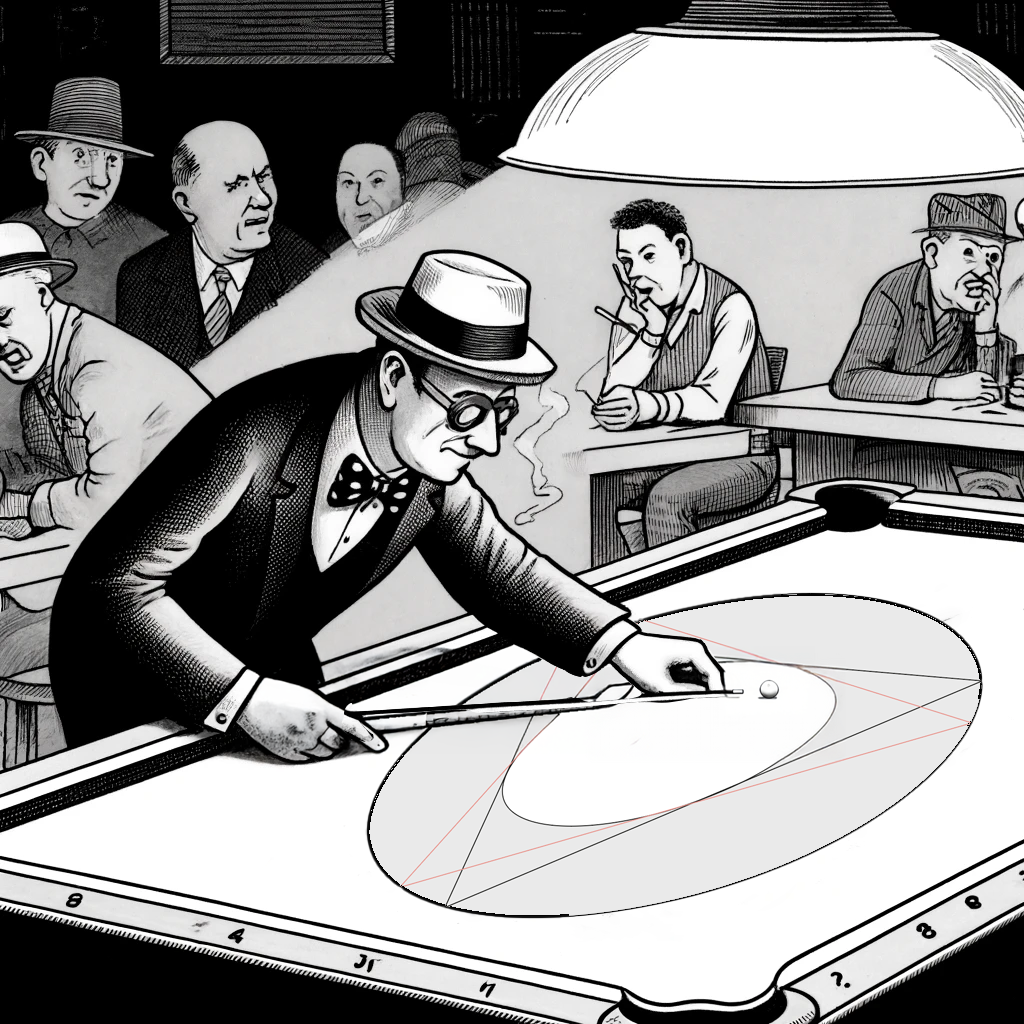
\includegraphics[width=0.8\textwidth]{07_BilliardsConicsPorism/BILLIARDS.png}
%}{Mike's understanding of Snell's law made him unbeatable,\\ but considerably slowed down the game}%
    }{}
    
    \IfFileExists{#1/imagefigure.tex}{%
        \imagefigure{
    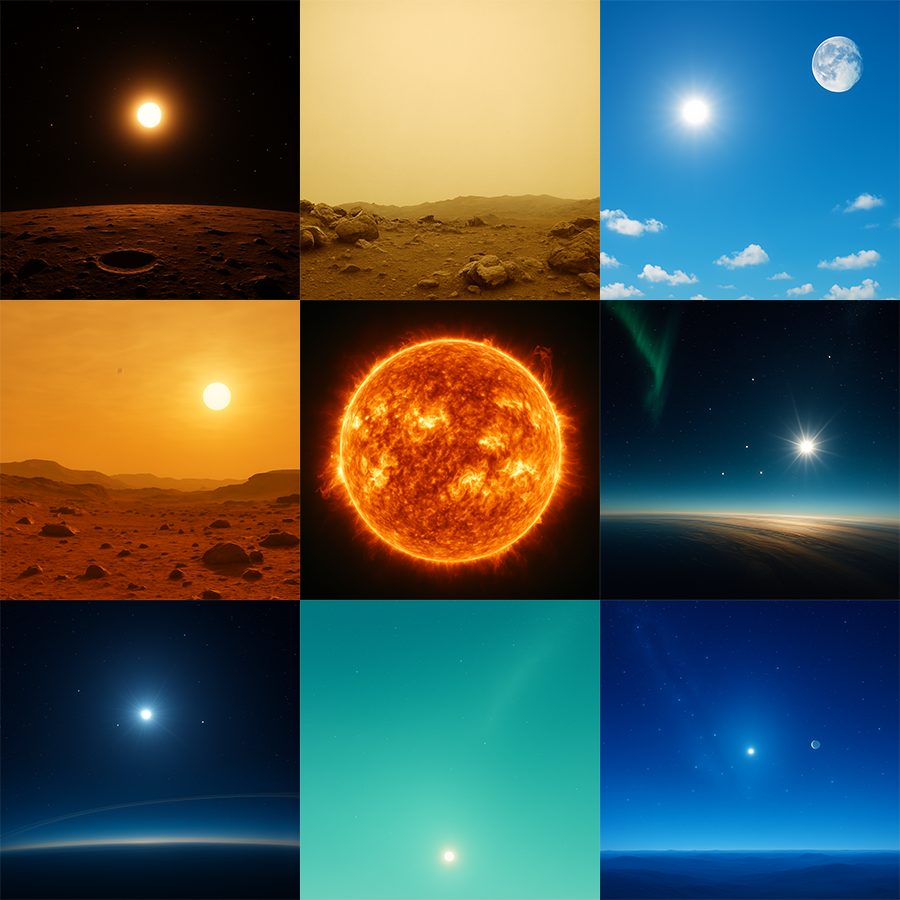
\includegraphics[width=0.8\textwidth]{27_PlanetarySkyColors/SKIES.png} 
}{
Nine simulated daytime skies from each planet in the Solar System, arranged heliocentrically around the Sun in a 3×3 grid. The rows (left to right, top to bottom) correspond to: Mercury, Venus, Earth; Mars, Sun, Jupiter; Saturn, Uranus, Neptune. Each panel reflects sky color, atmospheric scattering, and visible celestial features such as moons, rings, and the Sun’s apparent size, as modeled for surface or high-atmosphere observation.
}
%
    }{}

    % --- PAGE 9: Technical (exactly 1 page) ---
    \newpage
    \begin{technical}
{\Large\textbf{The 1914 Christmas Truce: Documentary Evidence}}\\[0.7em]

\noindent\textbf{Primary Source Analysis}\\[0.5em]
Unit war diaries, personal letters, and official directives establish the truce as a geographically constrained phenomenon distinct from its mythologized afterlife. Archival data reveal heterogeneous local interactions shaped by material conditions and institutional ambivalence.

\noindent\textbf{Methodological Considerations}\\[0.5em]
Wartime testimony presents epistemological challenges: censorship protocols, postal delays, and narrative contamination through press accounts. Battalion war diaries constitute the most reliable documentary substrate — compiled contemporaneously under military regulations (Field Service Regulations Part II, 1909). Personal correspondence requires triangulation against unit records to establish veracity. German sources (Kriegstagebücher) demonstrate parallel reliability hierarchies: regimental over personal, Saxon over Prussian units.

\noindent\textbf{Geographic Distribution}\\[0.5em]
Truces concentrated along 30 miles of BEF front in Flanders and northern France. Battalion records (London Rifle Brigade, Northumberland Hussars, 6th Gordon Highlanders) document cessation of fire, joint burials, gift exchanges, and carol singing. Saxon and Bavarian regimental reports corroborate these activities, noting English-speaking soldiers and prior civilian contact with Britain.

French-German interactions remain sparsely documented; French command structures prohibited fraternization. Belgian participation was minimal. Canadian involvement is apocryphal: the 24th Battalion CEF arrived France mid-1915. December 1914 BEF war diaries contain no Canadian unit references.

\noindent\textbf{Material Conditions}\\[0.5em]
Truce emergence correlates with specific environmental factors: waterlogged trenches (Ploegsteert sector), proximity enabling auditory contact (50–100 yards separation), and supply chain irregularities. Weather data (Meteorological Office archives) indicate unseasonable warmth 24–26 December: ground frost absent, facilitating movement. Static warfare's early phase — pre-gas, pre-continuous wire — permitted physical accessibility. The "live and let live" system (Ashworth, 1980) had embryonic precedent in localized breakfast truces and predictable artillery schedules.

\noindent\textbf{The Football Myth}\\[0.5em]
No battalion war diary from confirmed truce sectors records organized football. The sole contemporaneous reference — a Rifle Brigade doctor's letter in \textit{The Times} — mentions "a football match" without unit identification or details. Other testimonies describe "kickabouts" or aborted plans amid impassable terrain. Letters referencing play are second-hand or anecdotal.

The "3–2" scoreline appears in no primary materials, originating in postwar elaborations. Informal recreation occurred sporadically; organized matches between opposing sides remain undocumented.

\noindent\textbf{Command Response}\\[0.5em]
General Forrestier-Walker issued preemptive anti-fraternization orders 24 December 1914; German command followed 29 December. Neither pursued disciplinary action afterward. Officers joined their men in No Man's Land or ignored violations.

Documentary evidence reveals institutional ambivalence: II Corps (Smith-Dorrien) issued retrospective condemnations without prosecutions; 7th Division (Capper) acknowledged events without censure. German archival materials (Hauptstaatsarchiv Stuttgart) indicate parallel hesitancy — Kronprinz Rupprecht's Sixth Army headquarters recorded but did not punish infractions. This contrasts sharply with later French military justice: 1917 mutiny trials cited 1914 fraternization as aggravating precedent.

Christmas 1915: pre-planned artillery bombardments, court-martials of British officers Miles Barne and Iain Colquhoun. Haig annulled Colquhoun's sentence, but enforcement became policy. Future truces precluded through mandated hostility.

\noindent\textbf{Historiographical Arc}\\[0.5em]
British and German newspapers reprinted letters within days. Official histories (1918–1935) omitted the event. Scholarly recovery: 1960s onwards, concurrent with pacifist reinterpretations of WWI. The football myth proliferated through visual media: McCartney's "Pipes of Peace" (1983), Sainsbury's advertisement (2014).

The mythologization process exemplifies Hobsbawm's "invention of tradition": prosaic fraternization transformed into structured sporting event. Archival silence (1918–1960) enabled narrative drift. Post-1960s scholarship (Terraine, Ferro, Eksteins) established documentary parameters while popular culture elaborated counterfactual details. The truce functions as lieu de mémoire (Nora, 1984): actual events subordinated to commemorative utility.

\vspace{0.5em}
\noindent\textbf{References:}\\
Ashworth, T. (1980). \textit{Trench Warfare 1914–1918: The Live and Let Live System}. Macmillan.\\
Brown, M. (2007). \textit{Christmas Truce: The Western Front, December 1914}. Pocket.\\
Eksteins, M. (1989). \textit{Rites of Spring: The Great War and the Birth of the Modern Age}. Houghton Mifflin.\\
Ferro, M. (1973). \textit{La Grande Guerre 1914–1918}. Gallimard.\\
Hobsbawm, E. & Ranger, T. (eds.) (1983). \textit{The Invention of Tradition}. Cambridge UP.\\
Imperial War Museums. \textit{First World War Personal Letters Collection}.\\
National Archives UK. \textit{BEF Unit War Diaries, Dec 1914}.\\
Nora, P. (1984). \textit{Les Lieux de mémoire}. Gallimard.\\
Weintraub, S. (2001). \textit{Silent Night: The Story of the World War I Christmas Truce}. Plume.
\end{technical}


    % --- NO PAGE 10 EMPTY PAGE HERE ---
    % Empty verso pages are now added BEFORE each chapter (see top of \inputstory)
    % This prevents cumulative page drift and maintains 10-page alignment
    % Last chapter will not have trailing empty page


}

\definecolor{purplebackground}{RGB}{230,230,250} % Lavender/purple background
\newsavebox{\SideTextBox}
\newenvironment{SideNotePage}[2] % #1 = side text, #2 = image path
{%
  \clearpage
  \thispagestyle{empty}
  
  % Layout for 432x972pt PDFs within 5.5"×8.5" text area
  % Left: caption, vertical line separator, Right: centered image
  \vspace*{\fill}
  \noindent
  \begin{minipage}[c]{1.8in}
    \raggedright
    \footnotesize
    #1
  \end{minipage}%
  \hspace{0.1in}%
  \rule[-3.5in]{0.5pt}{7in}% vertical line separator
  \hspace{0.1in}%
  \begin{minipage}[c]{3.4in}
    \centering
    \includegraphics[width=3.2in,height=7.5in,keepaspectratio]{#2}
  \end{minipage}%
  \vspace*{\fill}
}
{%
  \clearpage
}





% Ensure technical environment doesn't break across pages
\AtEndEnvironment{technical}{\nopagebreak[4]}
